\documentclass[11pt,a4paper]{report}

\setcounter{tocdepth}{3}
\setcounter{secnumdepth}{3}

\usepackage[utf8]{inputenc}
\usepackage[margin=1in, a4paper]{geometry}
\usepackage{array}
\usepackage{blindtext}
\usepackage{titling}
\usepackage{xcolor}
\usepackage{ulem} % Custom underlining sizes
\usepackage{natbib} % For references
\usepackage{graphicx}
\graphicspath{ {./images/} } % Allows images to be imported
\usepackage{url}
\usepackage{float}
\usepackage{tabularx} % For tables

\usepackage{lastpage}
\usepackage{fancyhdr}


\renewcommand{\bibname}{References}

\setlength{\headheight}{13.6pt}

\usepackage{hyperref} % Allows contents page to be "clickable"
\hypersetup{
    colorlinks,
    citecolor=black,
    filecolor=black,
    linkcolor=black,
    urlcolor=black
}

% Defining colours
\definecolor{dark-green}{RGB}{00, 80, 00}
\definecolor{d-purple}{RGB}{80, 00, 80}
\definecolor{l-blue}{RGB}{207,226,243}
\definecolor{l-green}{RGB}{217,234,211}
\definecolor{l-red}{RGB}{244,204,204}
\definecolor{l-purple}{RGB}{217,210,233}
\definecolor{crimson-red}{RGB}{220, 20, 60}

\title{ \begin{Huge} \textbf{NEA Analysis Section} \end{Huge} }
\author{ \begin{LARGE} \textbf{Vedant Bhopatrao 12B}
\end{LARGE} }
\date{ \begin{large} \textbf{Monday 3rd May 2021}
\end{large} }

\pagestyle{fancy}
\fancyhf{}

% Header
\fancyhead[L]{\textsc{\nouppercase{\leftmark}}}
\fancyhead[R]{\textsc{\nouppercase{\rightmark}}}

% Footer
\fancyfoot[C]{Page \textbf{{\thepage}} of \textbf{\pageref{LastPage}}}

\begin{document}
    \maketitle
    \tableofcontents

\newpage
\chapter{Analysis}
\section{Description of the problem}
Many children and teens have lots of time to spare in their young lives, but what \textit{exactly} would be the best way to spend that time without \textit{wasting it on nothing} or having the constant feeling of boredom? \newline

\noindent \textit{One} way to spend that valuable time would be to play games with friends and family, to bond further over \textit{multiplayer} games of their interests. Especially during unprecedented times like the pandemic where social contact is limited, what better way to reconnect people online while maintaining distancing and having fun than by playing games online, with friends and family? \newline

\noindent But another problem that people have with a game like \textit{Carrom} is its portability. A king sized board weights at around 18 kilograms, which means it will be hard to move around not only in the house but also if you intend on taking it elsewhere. Not only does this present a problem to people who may not be capable of carrying heavy weights, but it can also be quite dangerous if the board gets damaged or gets accidentally slipped.  \newline

\noindent A Carrom boards are also pricey, coming at £60 to £120 - not everyone is able to afford the game. They are also easy to damage from scratches, which means the smoothness of the pieces moving won't be there if marks are left on the board from any damages. This can lead to a reduction in the game quality and could potentially mean a replacement in the board itself. \newline

\noindent Considering there are 19 total pieces (not including the striker), it is very easy to lose any one of these pieces. Would this problem occur if the physical aspect of the game was removed? \newline

\noindent A better solution to these physical problems would be to make the game playable in a way where none of these issues would occur. The best and easiest way to do with would be to make the game online to be played on a computer device. \newline

\noindent However, an online problem many people face is the amount of time spent looking at your system's display screen. A possible solution to this that can be provided are analytics, displaying how long you have played the game in total and your daily average length. This would help send reminders to the user, when they are close to reaching their average rate, telling them to take a break.

\section{Description of the project}
My project will be the computerised version of the game "Carrom". Carrom is a game that can be played by two or four people. Each person striker area is on each side of the board, and the turns proceed in clockwise order. If a user wants to play single player, they can play against the computer or go into a "practice" mode where they play by themselves to get used to the game.

\subsection{Basic rules}
\begin{itemize}
  \item The first turn is determined randomly, by the computer.
  \item If a player pockets no pieces or commits a foul, their turn is over and goes to the next player.
  \item It does not matter if a striker hits a piece or not, after it has been shot the players turn is over.
  \item If a player pockets an opponents piece, the piece goes to the opponent.
  \item Both two game modes refer to \textit{pocketing} a piece. This means to use the players striker to aim to shoot a piece into the corner where a hole is (on each corner of the board). However, the striker can also be used in a set boundary on each side of the players board, to limit the options of shots playable so it does not become too \textit{easy}.
\end{itemize}

\subsection{Fouls}
Here are examples of fouls that may occur during the game and their penalties:
\begin{itemize}
  \item A players own striker is pocketed. If this happens, the piece must return to the middle of the board and no points will be gained if they are in the game mode.
  \item If a user pockets their own piece into the corner, the player must return their piece to the middle of the board and the next turn is played out by the opponent. They will also lose the amount of points that the piece is worth.
  \item A player pockets all of the opponents pieces except the Queen. If this occurs, the game ends and the opponent wins.
\end{itemize}

\subsection{Main menu}
\subsubsection{Description}
\noindent Below listed are the options that will be displayed on the main menu. There are two different game modes in which Carrom can be played, which are further explained below.

\subsubsection{Demo}
\begin{itemize}
    \item Displays a tutorial to newcomers on how to play the game when playing the game for the first time.
\end{itemize}

\subsubsection{Practice}
\begin{itemize}
    \item Makes a private solo room to allow the end user to familiarise themselves with how the game works and with the program itself.
    \item Primarily used to gain practice and so the user becomes better at playing the game.
\end{itemize}

\subsubsection{VS Computer}
\begin{itemize}
    \item Allows the user to verse the computer for practice.
    \item In this mode statistics will not be recorded and the primary reason of this mode is to allow the player to have practice
\end{itemize}

\subsubsection{Game mode 1: Teams}
\begin{itemize}
    \item The first method is where each player has either 6 brown pieces or 6 black pieces along with a Queen, and the objective of the game is to see whoever can pocket all of the opponents pieces as fast as possible, with no time limits.
    \item This game mode is usually played by either 2 or 4 people. Turns are taking in clockwise direction.
    \item In this game mode, a player can win by using their striker to pocket all the enemy pieces first. However, the last two pieces that must be pocketed, in order, are the opponents Queen (in dark pink colour), and a regular piece of the opponent (either brown or black).
    \item If the last two pieces do not include the Queen, the opponent automatically wins the game. Also, if the last two pieces have been pocketed in the opposite order, then both pieces are returned to the middle of the board and stacked on top of each other and the game resumes.
    \item If a user pockets their own piece into the corner, the player must return their piece to the middle of the board and the next turn is played out by the opponent.
\end{itemize}

\subsubsection{Game mode 2: Point system}
\begin{itemize}
    \item The second method is where there are 12 pieces on the board, 6 are brown and the other 6 are black. The 6 brown pieces are all worth 2 points, whereas the 6 black pieces are worth one point.
    \item This game mode is usually played by 2 people. Turns are taking in clockwise direction.
    \item It is played as a \textit{"free-for-all"} game where both players are allowed to pocket any of the pieces, the main objective is to pocket as many pieces of possible and end up with the most amount of points.
    \item In this game mode, the objective is to try and pocket as many of the opponents pieces as possible, through the use of the players striker piece, under a time limit of 8 minutes, on each players end. After the time limit has been reached, whoever has accumulated the most amount of points through pocketing will be declared the winner.
\end{itemize}

\subsubsection{Summary}
\noindent These 3 different game modes (and a quit option) will be presented on the home screen menu, using a GUI (Graphical User Interface), when the user starts the program. From there, they can select which game mode they would like to proceed with, and the game mode will be selected and started through this. \newline

\noindent In regards to the complexity, I will be making the game online and multiplayer, so it be played with friends and family, using a peer to peer network model.

\section{Computational Methods}
The computational methods mentioned below will help me overall to produce a game in the shortest amount of time possible, while still making sure it is robust and has been created at an efficient rate with the least amount of bugs and errors.

\subsection{Decomposition}
\subsubsection{Description}
To solve the problem I must decompose it into smaller, individual problems that can be tacked one-by-one. This will increase efficiency in the time frame of the programs production and the work rate.
\subsubsection{Justification}
For example, I can treat each different feature as a separate module as self contained steps that I will solve individually. These may include but are not limited to; creating the board, impact of a striker hitting a piece, taking turns between the players, the main menu, connecting two people together and a timer limit in some of the game modes.

\subsection{Abstraction}
\subsubsection{Description}
Using abstraction will help me finish my program in a shorter amount of time since the creation process will be shorter, due to removing unnecessary elements to my game that do not contribute anything towards it.
\subsubsection{Justification}
For example, instead of focusing on the graphical details to each piece on the game, I can focus on the functionality and features it has instead. This will help in the development time of the program, as I will not need to spend extra time making it look fancy while still having the core functions of the game.

\subsection{Algorithms}
\subsubsection{Description}
Use of algorithms can help speed the process of starting and finishing a game. This will be all done by the computer and some algorithms can be reused at later points in the game, if there are point in the game where the same actions have been carried out multiple times.
\subsubsection{Justification}
For example, when starting a new game, the counters will be automatically in place and ready for the game to begin. Instead of making sure the striker is placed within its boundary limits, like in a physical game, the system will automatically configure it so it will be impossible for it go outside of the boundary line.

\subsection{Visualisation}
\subsubsection{Description}
GUI (Graphical User Interface) will be used and provided to the client so they can interact with the game more easily and have more enjoyment doing so.
\subsubsection{Justification}
My program will provide a GUI to allow the user to react to the game based on the chain of events that take place. This makes it easier for the end user to make decisions by simply \textit{clicking} on the option they would like to choose. The GUI will also be easier to test and spot for errors/bugs are they will be visually displayed, if it is a logical error, and program will not run, if it is a syntax error. The GUI that I will be using will be made from the Pygame module, which will gives me full control on the details that I would like to be displayed through the use of sprites to produce text and animation.

\subsection{Problem Recognition/Testing}
\subsubsection{Description}
I can look at previous examples of the game made online from which I can analyse to see what they did well in, what features they lack and the potential problems that have arose from the end users.
\subsubsection{Justification}
From the analysis, I can make a requirements table to make sure I can meet the criteria so my program will be expected to fix bugs that previous generations of Carrom online have. I can find these on the Internet and if there is a specific part which I cannot find, I can look into similar games with the same concept, such as Pool to further my analysis. This will help me keep the quality level of all parts the same, and to not have modules with different levels of quality in the way they were made.


\renewcommand{\ULdepth}{1.8pt}
\subsubsection{Traditional approach vs digital solution}
\begin{center}
\begin{tabular}{ | m{1.5em} | m{15em} | m{21.2em} | }
\hline
 \uline{\textbf{No.}} & \uline{\textbf{Physical}} & \uline{\textbf{Computerised}} \\
\hline
1 & Reorganise the whole field to start a new game & A preset can be made that wipes the current field and resets to the preset if a user wants to start a new game \\
\hline
2 & Player can accidentally move the position of a piece & Computer model will not allow both players to interact with the game at the same \\
\hline
3 & Board can become rough after multiple uses over a long period of time & Board will stay smooth constantly \\
\hline
4 & test & test \\
\hline
5 & test & test \\
\hline
\end{tabular}
\end{center}

\subsection{Performance Modelling}
\subsubsection{Description}

\subsubsection{Justification}
Performance modelling will help me keep track of the status of my program. This will help me to see which areas of the program are not meeting the standards as the rest of the code, so I can act upon them. This will prevent the game having different levels of quality between the features and allows me to check what works and what doesn't.


\subsection{Pattern Recognition}
\subsubsection{Description}
I can look at similar created product and compare them to mine.

\subsubsection{Justification}
By comparing to existing solutions, I am able to see what problems arose when they created their product, and from this I can learn what mistakes not to make during development. I can also look at reviews of the product, and see what features the users were expecting that were not there.


\subsection{Digital Data Storage}

\subsubsection{Description}


\subsubsection{Justification}



\section{Stakeholders}

\subsection{Description}
The majority of Carrom players come from a diverse age range group of people considering how ancient the game is, and how little it has changed over time. However, the game produced would be made online, and based on popularity from the audience of the age range of people that play games, the ideal target stakeholders would be people aged between ten and forty years old. Using a wide range group will help provide me useful information through the data collection methods, that will be provide me with the tools to produce a game that will not only suit a wide age range, but also the majority of the audience in both audiences of Carrom and video games. \newline

\noindent I have decided to hold two interviews and two surveys - each for either primary or secondary stakeholders. For both methods, I will listen to the feedback my client has given me, and note their criticisms in order to make the final product as satisfactory as possible for the end user. \newline

\noindent The interview will take place in a room where I ask the interviewee questions relating to the game in order to collect their views and feedback on how they would like the game to turn out and their expectations on what they want to see. The interviews conducted will allow me to receive responses in further depth and detail compared to other methods of data collection. \newline

\noindent For the second data collection procedure, I have used the survey method to reach a wider audience is through the use of a form I made using Google Forms. Unlike an interview where I am only able to collect responses from one person at a time, in a survey I am able to reach a wider audience and collect shorter answers that do not require detail all at the same time. \newline

\noindent My primary stakeholders will be my parents as they have had experience in playing Carrom physically since their childhood and I believe they will be able to give the best views on what features and functions to add because of this. The benefits of having them previously played the game allows me to have information on which areas of the game they might not have liked or what new and extra features they might want implemented. \newline

\noindent My secondary stakeholders will be friends who will not have played the game before. They can provide useful hindsight into which features they would think make the game more user friendly, and could suggest options of what to add to the game based on experiences from similar types of board games previously played.

\subsection{Interview 1 - Primary Stakeholders}


\subsubsection{Plan of the interview}
I will have an interview with my primary stakeholders - my parents, from which I can determine their requirements for the game and what features they would like implemented online from a traditional perspective. Considering they have played the games since their childhoods, I believe they will be able to suggest valuable inputs into the game and determine what problems that the physical game have had and whether or not it would be possible to patch them through the digital solution. Since they already know how to play the game, no information will need to be given during the interview about the game, but details about the format of the interview and how I will be developing the game online \textbf{will} be given pre-hand. \newline

\noindent From this interview, I can determine what aspect of the game, in their opinion, would be the hardest to program, and from there I can make a list on the priorities in the programming stages. I have planned the interview specifically to collect answers on what exactly the user is looking for when they decide to play the game online, and what features they would want to be added or removed from the traditional solution, so would provide a benefit to them playing digitally. \newline

\subsubsection{Interview transcript}
\begin{enumerate}
    \item \colorbox{l-blue}{Question:} \textcolor{blue}{How are you expecting the game to operate?}

    \colorbox{l-green}{Reasoning for question:} \textcolor{dark-green}{This will help determine the main requirements from the user, and will help me to set a criteria list on what features the game needs and what it doesn't need.}

    \colorbox{l-red}{Response received:} \noindent \textcolor{crimson-red}{"Well, I would expect it to operate how it would in real life. " \newline "The game should be easy to understand and easy to use. A self explanatory type. I would expect it to operate it the same way we used to play it in our childhood days. Because we knew all the rules of the game already." }

    \colorbox{l-purple}{Thoughts on response:} \noindent \textcolor{d-purple}{This answer will help me to determine the main priority when developing the game - that it should emulate functions very closely and similar to the physical game.}




    \item \colorbox{l-blue}{Question:} \textcolor{blue}{What should the resolution of the game be?}

    \colorbox{l-green}{Reasoning for question:} \textcolor{dark-green}{This will help determine the main requirements from the user, and will help me to set a criteria list on what features the game needs and what it doesn't need.}

    \colorbox{l-red}{Response received:} \noindent \textcolor{crimson-red}{"It should work the same way as we used to play earlier. It should be entertaining - utilising my time in a fun way. Extra new features I would not mind as long as"}

    \colorbox{l-purple}{Thoughts on response:} \noindent \textcolor{d-purple}{This answer will help me to}




    \item \colorbox{l-blue}{Question:} \textcolor{blue}{What colour scheme should I use for my game and why?}

    \colorbox{l-green}{Reasoning for question:} \textcolor{dark-green}{Asking my stakeholder specific questions like these helps me to create a criteria list on key appearances of they game that they would like, which reduces times spent for decisions made by myself on their behalf.}

    \colorbox{l-red}{Response received:} \noindent \textcolor{crimson-red}{"Well I am imagining a carrom board I would expect a similar colour scheme to that of a chess board so dark brown or tans , whites, red. Brown to tan." \newline "Not too bright, neutral colours. It should be similar to how it is played in real life. I would not mind any colour as long it is vibrant and not too strong.
It should not be too bright or giving strain on my eyes so I will be able to play for longer times. "}

    \colorbox{l-purple}{Thoughts on response:} \noindent \textcolor{d-purple}{test}



    \item \colorbox{l-blue}{Question:} \textcolor{blue}{What critical features do you expect to be included in the game that are a must and why?}

    \colorbox{l-green}{Reasoning for question:} \textcolor{dark-green}{This question allows me to see in detail what exact features they would expect to see included in the game.}

    \colorbox{l-red}{Response received:} \noindent \textcolor{crimson-red}{"- When you flick the striker it should be on the line
- If you hit your own piece into the hole, it should count as a point for the other team just like it would for any game
- Keeping score of the points based on the pieces
- In the menu it should show how much each piece is worth so you know that and are aware of that so during the game you would aim for the pieces that are worth more
- Not really on the pieces, but at the start it should show a small preview or a key of how much each piece is worth if you are playing in the points based mode" \newline \newline "- Clues or tips on the next move to make
- Steps or guides on how to play the game
- It should work as a carrom board in real life
- Easy to use and user friendly menu.
- Demo to make it easier to understand for beginners"}

    \colorbox{l-purple}{Thoughts on response:} \noindent \textcolor{d-purple}{Based on this answer, I can tailor my game to suit my clients needs}




    \item \colorbox{l-blue}{Question:} \textcolor{blue}{What feature would you want that makes the experience more fun in Carrom?}

    \colorbox{l-green}{Reasoning for question:} \textcolor{dark-green}{This question allows me to know what personally they would want to see in the game if it was only played by them, rather than a larger audience.}

    \colorbox{l-red}{Response received:} \noindent \textcolor{crimson-red}{"Challenge aspect, a handicap where you have to achieve (add challenges to the game so it doesn't become repetitive)
- e.g. a time limit for each player turn.
- time limit can decrease in each round (starting round can start with 2 minutes for each turn, after each round, time limit decreases by 10 seconds)
- total time limit will decrease after each round
- Time limit works better in real life, as you can have a timer on the screen which means it is easier to keep track of" \newline \newline "- If I make a move, the computer can intervene and say a better move that I could have possibly done"}

    \colorbox{l-purple}{Thoughts on response:} \noindent \textcolor{d-purple}{test}





    \item \colorbox{l-blue}{Question:} \textcolor{blue}{What features do you think the game should include that might not be that important and why?}

    \colorbox{l-green}{Reasoning for question:} \textcolor{dark-green}{From this question I will be able to know what functions I should prioritise and which I can keep to nearer the end of development, which might not be that important.}

    \colorbox{l-red}{Response received:} \noindent \textcolor{crimson-red}{"An arrow for the striker in which direction it is pointing at; a visual representation to make it easier to aim. Timer at the top for the time limit for each player." \newline "- Achievements and statistics of previous games
- Stats about the user so world records can be hold (guinesse world records, etc)
- Self player statistics; winning and losing stats. For the persons own knowledge. (LIKE BEDWAR STATS)
- Takes a lot of time for the game to finish to add a time limit"}

    \colorbox{l-purple}{Thoughts on response:} \noindent \textcolor{d-purple}{test}




    \item \colorbox{l-blue}{Question:} \textcolor{blue}{In your opinion, what specific features would you like to see implemented within the game?}

    \colorbox{l-green}{Reasoning for question:} \textcolor{dark-green}{This question allows me to know what personally they would want to see in the game if it was only played by them, rather than a larger audience.}

    \colorbox{l-red}{Response received:} \noindent \textcolor{crimson-red}{"Force counter to show how much force you are putting on the piece so you can predict how far the piece will move" \newline "- Give the point to the opponent if a player self pockets their piece into the corner of the board
- Time limits
- Library of moves which a player can perform
- Levelling system; once they reach level 10 for example, they get a guide of a professional moves which they can do
- After a game or two, can get the user to fill out a survey/form asking their experiences and suggestions on what they would like to see added (their review basically)
- In real life, the counters can be flicked from the power of the striker, which is not supposed to normally happen and I do not like, so I would like to see the game avoid this in the digital solution
- I would like to add a point counter, so I can see the amount of points I have in total at the point in time
- I would like to add a pieces pocketed on both sides counters. White pieces and black pieces. Queen in pink colour, striker can be any colour."}

    \colorbox{l-purple}{Thoughts on response:} \noindent \textcolor{d-purple}{test}





    \item \colorbox{l-blue}{Question:} \textcolor{blue}{Have you used any similar solutions before? If so, what do you like from it?}

    \colorbox{l-green}{Reasoning for question:} \textcolor{dark-green}{This question tell me whether the stakeholder would be experiencing a game produced digitally for the first time, or if they have experience with similar games being played. If that is the case, I can collect information on key details to the functions they like, and possibly attempt to implement it within my solution, if possible.}

    \colorbox{l-red}{Response received:} \noindent \textcolor{crimson-red}{"Yes, I have played 8 ball pool and Golf before." \newline "Yes, I have played Wii Sports on Nintendo and Golf before."}

    \colorbox{l-purple}{Thoughts on response:} \noindent \textcolor{d-purple}{test}



    \item \colorbox{l-blue}{Question:} \textcolor{blue}{Would you like the game to be online so you can play with friends on the same network and why and what benefit does this provide to you?}

    \colorbox{l-green}{Reasoning for question:} \textcolor{dark-green}{This question allows me to see their thoughts on one of the game modes that will be added.}

    \colorbox{l-red}{Response received:} \noindent \textcolor{crimson-red}{"You can connect with people online; friends and family. Who might not be in the same area. For practice; you can play against random people and still have the same enjoyment. Doesn't have to be against computer/ the bot this way " \newline "- Online with friends or with the computer itself
- Demo friendly
- For the first few games, when using the cursor to hover over a piece, information should be displayed about the function of the piece
- Yes, because with online it gives more advantages, as you do not need the game in front of you. You can play on demand, with social distancing."}

    \colorbox{l-purple}{Thoughts on response:} \noindent \textcolor{d-purple}{test}



    \item \colorbox{l-blue}{Question:} \textcolor{blue}{How would you like the main menu to look like and what critical features do you expect from it?}

    \colorbox{l-green}{Reasoning for question:} \textcolor{dark-green}{From this I can see how I should be designing the main menu, whether it be in a specific way that the stakeholders prefers or not.}

    \colorbox{l-red}{Response received:} \noindent \textcolor{crimson-red}{"Big play button at the centre. Settings; audio level, help, contact. Rules button; shows actual rules and how to play the game. Visual representation to show how the game works rather than blocks of text, animation shown when you click the rules button" \newline "I would like to see the Carrom board with the striker and pieces on the main menu.
I should be able to click on the screen to show me what the game can offer me. (Demo, practice, start, game score and finish functions.)"}

    \colorbox{l-purple}{Thoughts on response:} \noindent \textcolor{d-purple}{test}




    \item \colorbox{l-blue}{Question:} \textcolor{blue}{Would you like a login system to save your progress and so multiple people can play on a device?}

    \colorbox{l-green}{Reasoning for question:} \textcolor{dark-green}{This question allows me to see their thoughts on one of the game modes that will be added.}

    \colorbox{l-red}{Response received:} \noindent \textcolor{crimson-red}{"When you have a login system that keeps track of your score, you can have a leaderboard. Bronze, silver, gold, that keeps track of how good your abilities are at the game which can keep track of your progress. Adds a further level of competitiveness to see yourself compared against other players with different ranks" \newline "- I can see my last progress and try to excel myself from the previous game
    - Yes so if I leave the game I am able to return to the game after a while while taking a break myself so I can come back to play the game after a while. To reduce playing the game for a long time.
    - Progress can be saved unlike irl, where if a piece is mistakenly moved by accident or something, then you don't know the original piece of where it was before, therefore it would be better to have it online where you can't make accidental mistakes like this."}

    \colorbox{l-purple}{Thoughts on response:} \noindent \textcolor{d-purple}{test}



    \item \colorbox{l-blue}{Question:} \textcolor{blue}{Would you like a leaderboard system to compete against other people?}

    \colorbox{l-green}{Reasoning for question:} \textcolor{dark-green}{This question allows me to see their thoughts on one of the game modes that will be added.}

    \colorbox{l-red}{Response received:} \noindent \textcolor{crimson-red}{"Yes, because it's a lot more fun to challenge yourself to see how good you are at the game. When normally you are against a bot" \newline "Yes, because it's a lot more fun to challenge yourself to see how good you are at the game. When normally you are against a bot
    - Yes, so I can see the progress of myself and to have some friendly competition against people that I have made friends with online on the game.
Yes, so I can see how to improve my game next time."}

    \colorbox{l-purple}{Thoughts on response:} \noindent \textcolor{d-purple}{test}



\end{enumerate}

\subsubsection{Interview Summary}
Overall, this interview has helped provide me a useful hindsight into what people that have played Carrom before would want specifically. Although the interview was only with one person and therefore would not represent the majority of peoples opinions, it is still able to provide common answers and suggestions into their likings. \newline

From this I have learnt how the primary stakeholders would expect the end product to turn out and look like, from which I can make a set of requirements than I would need to meet once the development of the program has begun.






\subsection{Interview 2 - Secondary Stakeholders}

\subsubsection{Plan of the interview}
I will have an interview with my secondary stakeholders, (people who did not know how Carrom works before), and discuss with them what requirements and criteria they would like the game to meet. \newline

\noindent I will format the interview into a two-part section; in the first part they will receive a debriefing into the main functions of the game, followed by a few questions regarding the features they would like to see implemented. These questions will expect answers to be quite broad considering the lack of information that the users have about the program, from which can be condensed and broken down further for specific details that they would like which we should expect to find in the second part of the interview.

In the second part, they will receive more in-depth detailed information into the game after which I will ask more specific questions, such as what colour scheme they would like to see the game in, how they would like the main menu user interface to look like, etc. \newline

\noindent After the interview, I should determine what functions they would like to see implemented into the game, and what exactly they are looking forward to playing within the game. From this, I will be able to see the different viewpoints and perspectives both sides of stakeholders and the main benefit of the secondary stakeholders is the valuable information that they can provide me with will enable me to reach and make the game accustomed to the target consumers likings.  \newline

\noindent At the end of the interview, I will be able to determine what exactly the client is looking for in the game to satisfy their needs and this way the program will turn out in a way they expected and wanted. This is appropriate to their needs as \newline


\subsubsection{Interview transcript}
\begin{enumerate}
    \item \colorbox{l-blue}{Question:} \textcolor{blue}{How are you expecting the game to operate?}

    \colorbox{l-green}{Reasoning for question:} \textcolor{dark-green}{This will help determine the main requirements from the user, and will help me to set a criteria list on what features the game needs and what it doesn't need.}

    \colorbox{l-red}{Response received:} \noindent \textcolor{crimson-red}{"test"}

    \colorbox{l-purple}{Thoughts on response:} \noindent \textcolor{d-purple}{This answer will help me to}

    \item \colorbox{l-blue}{Question:} \textcolor{blue}{How are you expecting the game to operate?}

    \colorbox{l-green}{Reasoning for question:} \textcolor{dark-green}{This will help determine the main requirements from the user, and will help me to set a criteria list on what features the game needs and what it doesn't need.}

    \colorbox{l-red}{Response received:} \noindent \textcolor{crimson-red}{"test"}

    \colorbox{l-purple}{Thoughts on response:} \noindent \textcolor{d-purple}{This answer will help me to}

    \item \colorbox{l-blue}{Question:} \textcolor{blue}{How are you expecting the game to operate?}

    \colorbox{l-green}{Reasoning for question:} \textcolor{dark-green}{This will help determine the main requirements from the user, and will help me to set a criteria list on what features the game needs and what it doesn't need.}

    \colorbox{l-red}{Response received:} \noindent \textcolor{crimson-red}{"test"}

    \colorbox{l-purple}{Thoughts on response:} \noindent \textcolor{d-purple}{This answer will help me to}


\end{enumerate}

\subsubsection{Interview 1 summary}
Overall, this interview has helped provide me a useful hindsight into what I should and should not do.


\subsection{Survey 1 - Primary Stakeholders}

\subsubsection{Plan of Survey}

I have formatted the survey into three separate sections: short questions (mainly used as a poll), medium response answers and long response answers. I have displayed this information clearly on the starting screen to provide the users information on what to expect throughout completing the survey and overall this makes it easier for the user to navigate through the questions.

In the short questions I have asked general type questions such as whether they think playing games provides them enjoyment, from which you can see the outcome of the survey below.

\subsubsection{Survey Results}


\subsubsection{Survey Summary}


\subsection{Conclusion}
From these methods of data collection, I have understood the




\subsection{Survey 2 - Secondary Stakeholders}

\subsubsection{Plan of Survey}

I have formatted the survey into three separate sections: short questions (mainly used as a poll), medium response answers and long response answers.

In the short questions I have asked general type questions such as whether they think playing games provides them enjoyment, from which you can see the outcome of the survey below.

\subsubsection{Survey Results}



\subsubsection{Survey Summary}



\section{Research}

\subsection{Existing solutions}
All of the existing solutions currently available are acceptable, but they do not provide a viable solution

\subsection{Carrom King}
\subsubsection{Description}
Carrom King is a digital version of the original game Carrom made available on the iOS and Android platforms that allows users to connect to each other and simulate the real life experience as close as possible.

The games main focus during development was to bring the experience of playing it digitally as close as possible to playing it with friends and family virtually.

It is a user friendly application that provides a solution to allow users to connect to each other to an online server to play together abroad.

The theme is very user friendly as it provides vibrant and joyful colours and the game itself it presented in a three dimension way. Its main platform is for people to play on mobile devices and presents itself as a solution to people who may not necessarily have a computer.

The design of the game is made to a high standard and it feels very realistic when playing.

Overall, the existing solution is almost flawless.
However, the demo complicates some of the controls, and instead should have forced the user to show the available controls rather than just displaying a text of where the controls are.



\subsubsection{Screenshots}

\begin{figure}[H]
\caption{Screenshot of the main menu in Carrom King}
\begin{center}
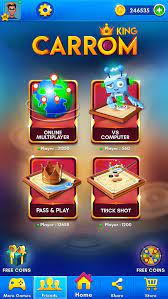
\includegraphics[width=0.5\textwidth]{images/analysis/carromking-menu.jpg}
\end{center}
\end{figure}

\begin{figure}[H]
\caption{Screenshot of a game in Carrom King}
\centering
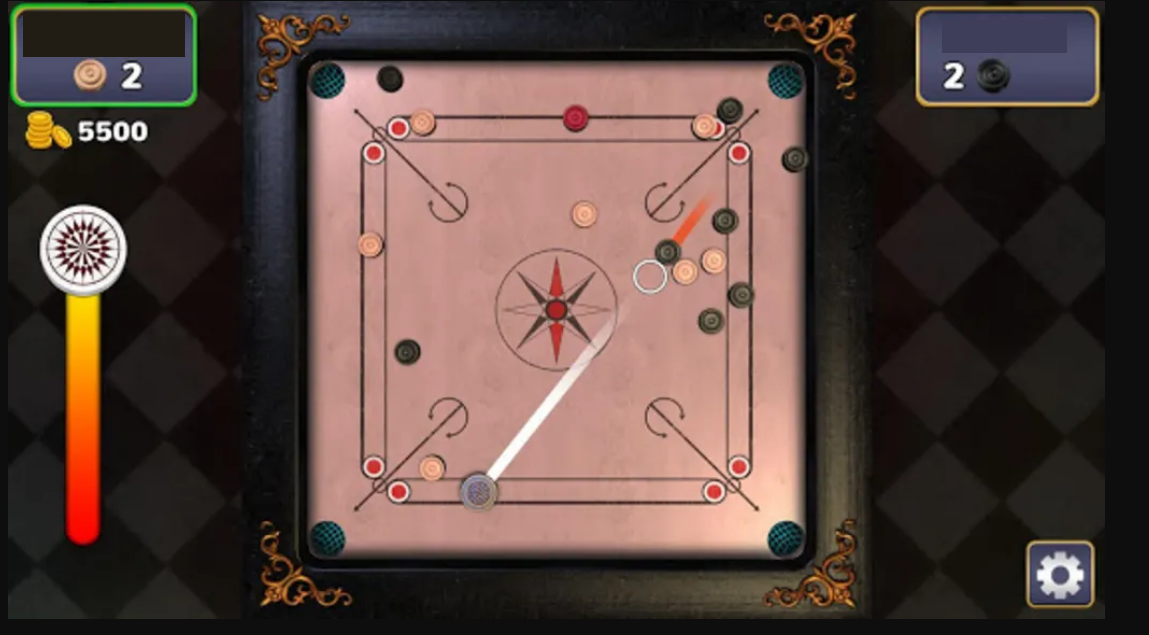
\includegraphics[width=0.5\textwidth]{images/analysis/carromking-ingame.png}
\end{figure}


\subsubsection{Reviews}

\subsubsection{Features}
\begin{enumerate}
    \item \textbf{Multiplayer Game Modes}
    \begin{itemize}
        \item Test
    \end{itemize}

    \item \textbf{Play with Friends}
    \begin{itemize}
        \item Test
    \end{itemize}

    \item \textbf{Single Player Offline Mode}
    \begin{itemize}
        \item Play against the Computer AI
        \item Play with people in the same house, as pass and play
    \end{itemize}

    \item \textbf{Cosmetics and Rewards}
    \begin{itemize}
        \item Test
    \end{itemize}

\end{enumerate}


\subsubsection{Conclusion}
From these data collection methods, I have learnt the


\subsection{Carrom Friends}


\subsubsection{Description}
Carrom Friends is an real-time, online carrom board game available on Android only. The solution aims to recreate a replica of the traditional game of Carrom played so it's exactly like my solution.


\subsubsection{Screenshots}

\begin{figure}[H]
\caption{Screenshot of the main menu in Carrom Friends}
\begin{center}
    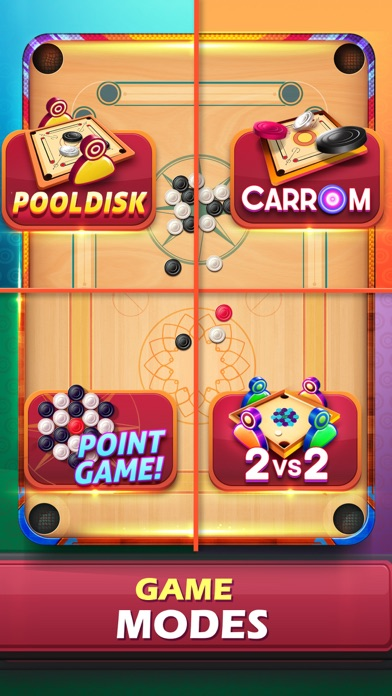
\includegraphics[width=0.5\textwidth]{images/analysis/carromfriends-menu.jpg}
\end{center}
\end{figure}

\begin{figure}[H]
\caption{Screenshot of a game in Carrom Friends}
\begin{center}
    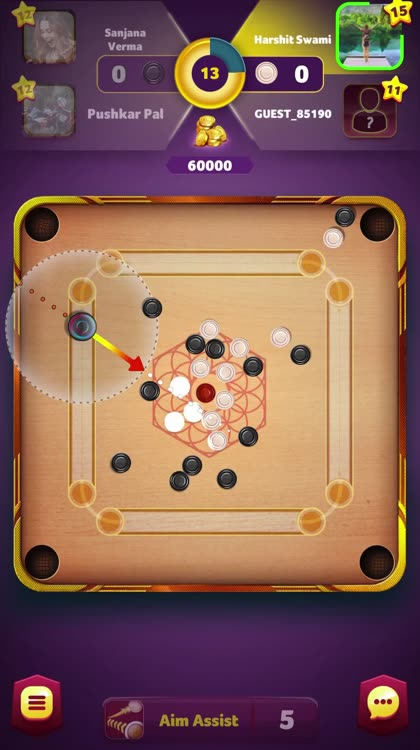
\includegraphics[width=0.5\textwidth]{images/analysis/carromfriends-ingame.jpg}
\end{center}
\end{figure}

\subsubsection{Reviews}

\subsubsection{Features}

\noindent It has 6 main features which are:

\begin{enumerate}
    \item \textbf{Connect with Facebook} \newline
Allows you to sync your progress online with Facebook, connect with people online, and unlock achievements through there.

    \item \textbf{In-Game Friends} \newline
This allows you to add people as friends within the game.

    \item \textbf{Carrom Mode} \newline
Normal Carrom Mode

    \item \textbf{Pool Disc} \newline


    \item \textbf{2v2} \newline
Allows you to play with friends in teams against other virtual players online.

    \item \textbf{Offline Mode} \newline
Allows you to play by yourself to gain practice.


\end{enumerate}


\subsubsection{Conclusion}

\subsection{8 Ball Pool}

\subsubsection{Description}
8 Ball Pool is a pool-based game played on a table with six pockets, cue sticks, and sixteen balls. It is usually played as a two-player game where one player has to pocket balls which are numbered between one to seven, and are solid colours, and the second player has to pocket balls numbered between nine to fifteen, which are striped. After all of each players ball have been pocketed, the final black coloured ball must be pocketed in order to win the game. \newline

\noindent It is a very entertaining game, with a strong vibrant metallic red, orange, and black theme to it.

\subsubsection{Reviews}
After reading reviews of the game from the Google Play Store, the majority seem to agree that it has been developed to be user-friendly and the users find it easy to navigate through the menus which shows that it has been well designed. They are also able to connect with friends and play with each other online, and are able to experience it similarly to how it would be played physically, in terms of connectivity. Although there were lots of positive reviews, there were also some negatives which criticised the way the developers implemented the game mechanics, and the bugs that they encountered due to this.  Multiple users seemed to have the same issue, which they expressed through the review on how changing the power levels for the cue affected the positioning of the where the stick was placed, which caused wastage of time, having to realign the cue again, and ultimately led the main factor of their loss, which kept building up as they play more and more. \newline

\noindent Another issue that \newline

\noindent A possible reason as to why this issue may not have been picked up earlier could be due to lack of testing after the end product had been created, to which the developer teams have solved this issue is by responding to the reviews. This is a feature that I could implement within my solution, perhaps ask to user whether they would like to fill out a quick, simple and short survey or review on features they thought were well implemented, and certain aspects of the game they would like to see improvements in. \newline

\subsubsection{Screenshots}

\begin{figure}[H]
\caption{Screenshot of the main menu in 8 Ball Pool}
\begin{center}
    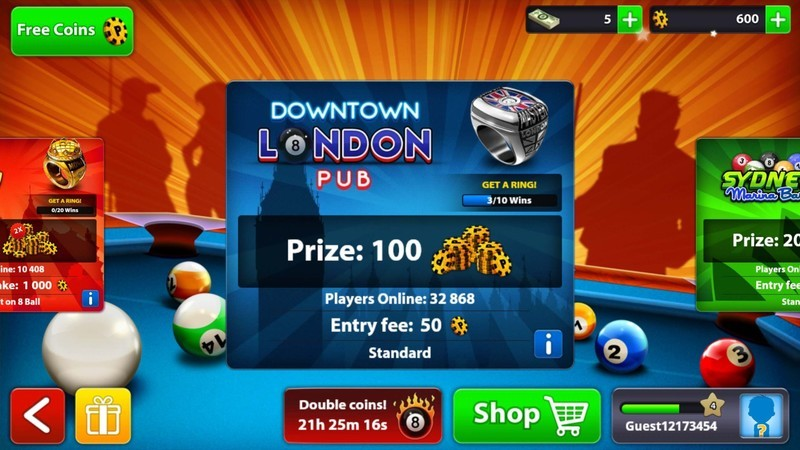
\includegraphics[width=0.5\textwidth]{images/analysis/8ballpoolmainmenu.jpg}
\end{center}
\end{figure}

\begin{figure}[H]
\caption{Screenshot of a game in 8 Ball Pool}
\begin{center}
    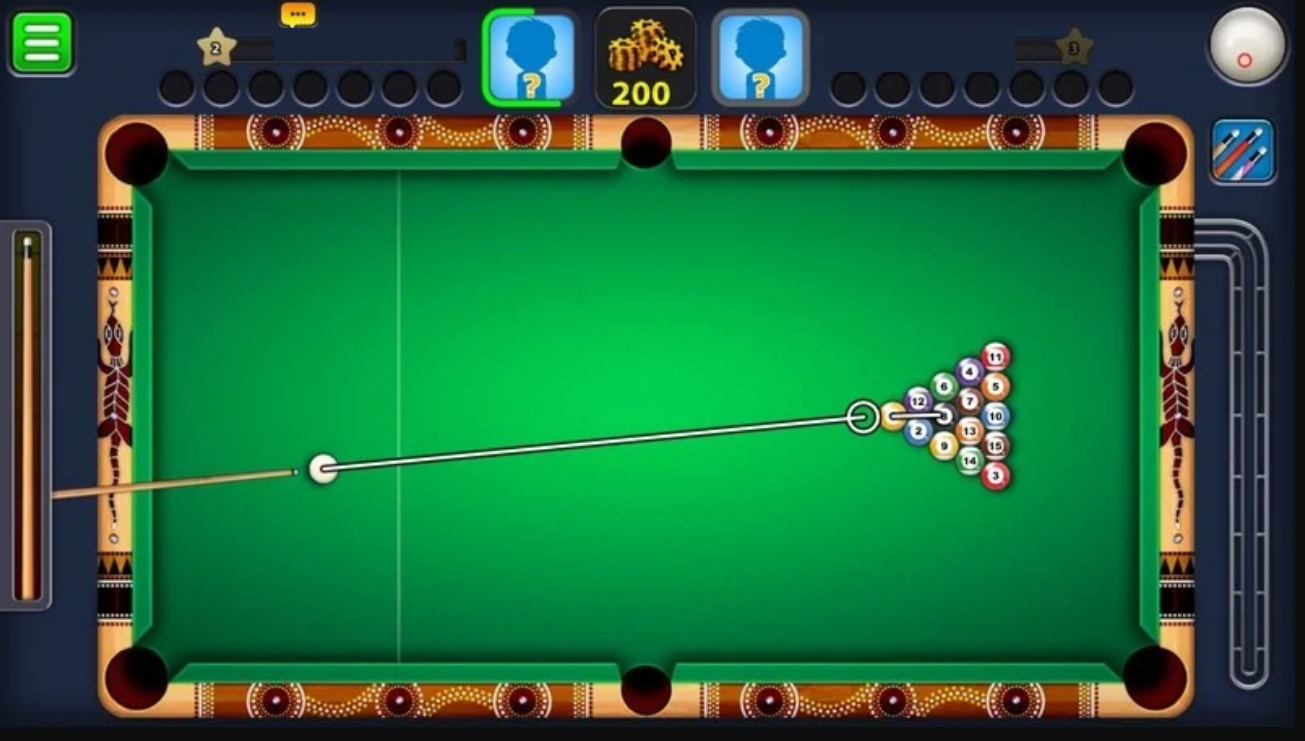
\includegraphics[width=0.5\textwidth]{images/analysis/8ballpoolingame.png}
\end{center}
\end{figure}


\subsubsection{Features}

\begin{enumerate}
    \item \textbf{Tournaments}
    \newline Participate in tournaments

    \item \textbf{Pool Coins and Exclusive Items}
    \newline Earn coins to buy cosmetics while playing

    \item \textbf{Challenge your Friends}
    \newline Play with friends

    \item \textbf{Level Up}
    \newline Level up to win exclusive rewards

    \item \textbf{iMessage Play Integration}
    \newline Play with friends through the "Messages" app, where the game will be integrated

    \item \textbf{Pro Membership}
    \newline Gain exclusive perks through having a membership


\end{enumerate}

\subsubsection{Conclusion}


\subsection{Snooker Stars}


\subsubsection{Description}
Snooker Stars is a 3D online game that strives to become the most realistic Snooker game that can be played digitally. It is available on the Google Play Store for Android devices, and provides a solution to having the feeling of playing snooker with friends or family online.

\subsubsection{Reviews}
Most reviews overall say that

Although there are some good reviews, there are also some negatives saying that the game is not optimised enough for all devices. Multiplayer is also a problem, as the connectivity between the players


\subsubsection{Screenshots}

\begin{figure}[H]
\caption{Screenshot of the main menu in Snooker Stars}
\centering
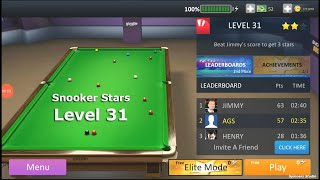
\includegraphics[width=0.5\textwidth]{images/analysis/snookerstars-mainmenu.jpg}
\end{figure}

\begin{figure}[H]
\caption{Screenshot of a game in Snooker Stars}
\centering
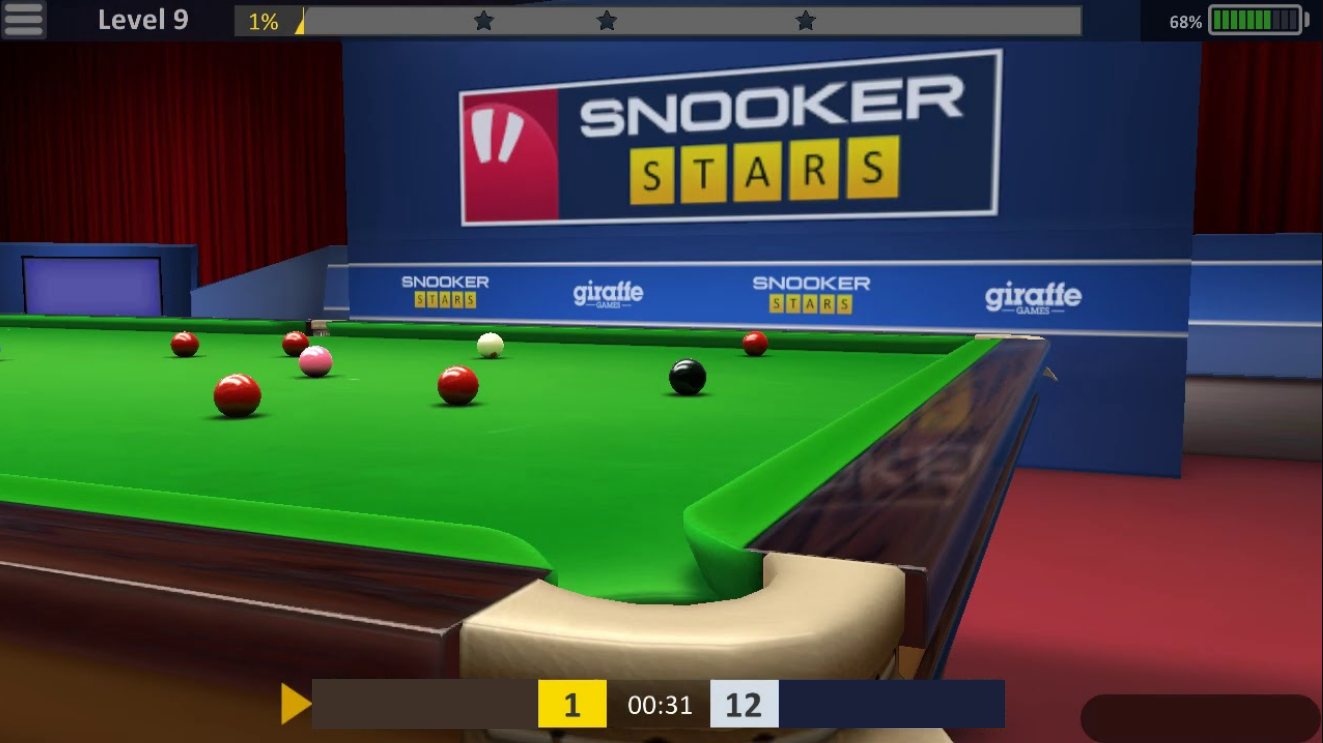
\includegraphics[width=0.5\textwidth]{images/analysis/snookerstars.png}
\end{figure}

\subsubsection{Features}
It has six main features that they take pride in creating such as:

\begin{enumerate}
    \item \textbf{Real life experience of playing snooker }
    \newline The game is in three-dimensions, allowing players to

    \item \textbf{In-built physics engine}
    \newline Developers made their own engine to

    \item \textbf{Advance your sports career}
    \newline Training mode to practice your skills to get better

    \item \textbf{Head-to-Head online matches}
    \newline Allows the players to verse random online people to practice or play with

    \item \textbf{World online leagues}
    \newline Allows the user to participate in world league to compete against others players around the world in a tournament

    \item \textbf{Add friends}
    \newline Allows you to play multiplayer with friends and family. This

    \item \textbf{Creating your own challenge}
    \newline This mode allows any user to create their own form of playing the game

\end{enumerate}

\subsubsection{Conclusion}


\subsection{Real Snooker 3D}

\subsubsection{Description}
Real Snooker 3D is a game that can be played on a mobile device. It is available on both the Google Play Store for Android, and the App Store for iOS.

\subsubsection{Reviews}
The average rating for the game is 4.4 stars. Although most reviews are good, some are very criticise in terms of the game mechanics as people complain that it is not very similar to how it would be played in real life.


\subsubsection{Screenshots}

\begin{figure}[H]
\caption{Screenshot of a game in Real Snooker 3D}
\centering
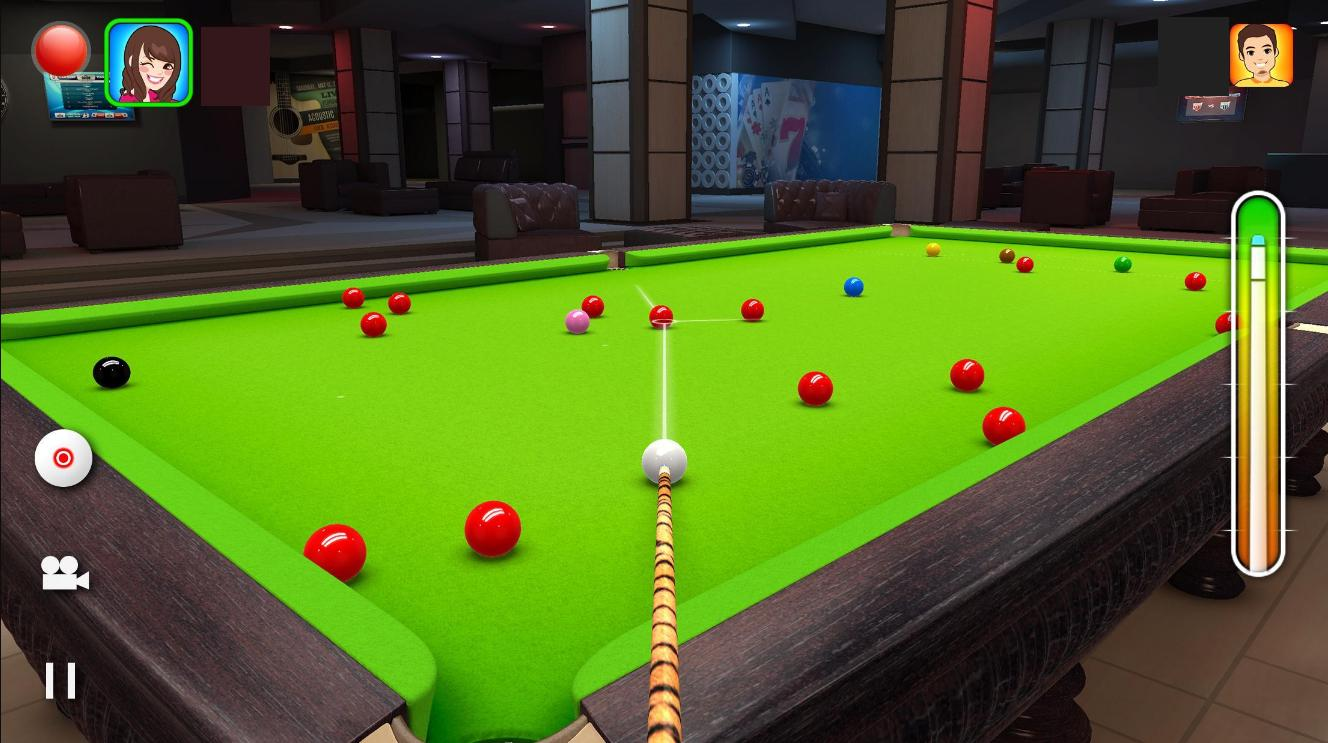
\includegraphics[width=0.5\textwidth]{images/analysis/realsnooker3dingame.jpg}
\end{figure}


\begin{figure}[H]
\caption{Screenshot of the main menu in Real Snooker 3D}
\centering
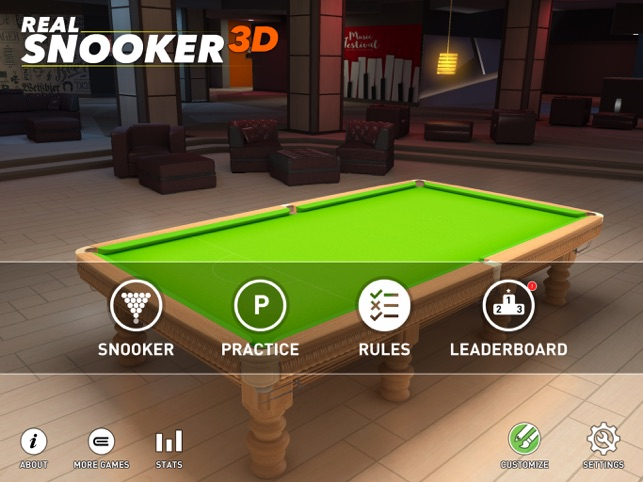
\includegraphics[width=0.5\textwidth]{images/analysis/realsnooker3dmenu.jpg}
\end{figure}


\subsubsection{Features}

\begin{enumerate}
    \item \textbf{Snooker Mode / Practice Mode}
    \newline Practice mode

    \item \textbf{Play with Computer}
    \newline Play against the AI where you can select the difficulty of the level to practice more

    \item \textbf{Play with Friends}
    \newline Play with friends online

    \item \textbf{Character Selection}
    \newline Choose a character to play as

    \item \textbf{Table Choice Selection}
    \newline Able to customise the appearance of what the snooker table looks like

    \item \textbf{3D graphics}
    \newline Beautiful graphics allowing the player to gain a more realistic perspective of how the game would be played physically
\end{enumerate}

\subsubsection{Conclusion}


\subsection{Overall Summary}

All five existing solutions that I have researched all



\section{Key features of the proposed solution}

text text text text text text text text text text text text text text text text text text text text text text text text text text text text text text text text text text text text text text text text text text text text text text text text text text text text text text text text

\begin{center}
\begin{tabular}{ | c | m{11em} | m{11em} | m{11em} | }
\hline
 \textbf{Requirement} & \textbf{Desirable} & \textbf{Acceptable} & \textbf{Failure} \\
\hline
Usability & Should work & test & test \\
\hline
Input & All inputs are functioning & test & test \\
\hline
Processor & Should be able to run on lower ends laptops & test & test  \\
\hline
Output & Should not have any logical or syntax errors, and output correctly & test & test  \\
\hline
\end{tabular}
\end{center}






\section{Software/Hardware requirements}

\subsection{Software requirements}
\begin{tabular}{|m{4.5em}|m{35em}|}
    \hline
    Software & Justification \\
    \hline
    Windows & Idk \\
    \hline
\end{tabular}


\subsection{Peripheral requirements}
\begin{center}
\begin{tabular}{ | m{4.5em} | m{35em} |}
    \hline
    Peripheral & Justification \\
    \hline
    Windows & \\
    \hline
\end{tabular}
\end{center}

\subsection{Hardware requirements}
\begin{center}
\begin{tabular}{ | m{4.5em} | m{35em} | }
    \hline
    Hardware & Justification \\
    \hline
    Windows & \\
    \hline
\end{tabular}
\end{center}



\section{Success Criteria}

\subsection{Input requirements}
\begin{center}
\begin{tabular}{ | c | m{18em} | m{18em} | }
\hline
 \textbf{No.} & \textbf{Criteria} & \textbf{Justification} \\
\hline
1 & test & test \\
\hline
2 & test & test \\
\hline
3 & test & test \\
\hline
\end{tabular}
\end{center}

\subsection{Processing requirements}
\begin{center}
\begin{tabular}{ | c | m{18em} | m{18em} | }
\hline
 \textbf{No.} & \textbf{Criteria} & \textbf{Justification} \\
\hline
1 & test & test \\
\hline
2 & test & test \\
\hline
3 & test & test \\
\hline
\end{tabular}
\end{center}

\subsection{Design requirements}
\begin{center}
\begin{tabular}{ | c | m{18em} | m{18em} | }
\hline
 \textbf{No.} & \textbf{Criteria} & \textbf{Justification} \\
\hline
1 & test & test \\
\hline
2 & test & test \\
\hline
3 & test & test \\
\hline
\end{tabular}
\end{center}


\section{Limitations}

\begin{center}
\begin{tabular}{ | c | m{18em} | m{18em} | }
\hline
 \textbf{No.} & \textbf{Limitation} & \textbf{Justification} \\
\hline
1 & test & test \\
\hline
2 & test & test \\
\hline
3 & test & test \\
\hline
4 & test & test \\
\hline
5 & test & test \\
\hline
6 & test & test \\
\hline
7 & test & test \\
\hline
8 & test & test \\
\hline
9 & test & test \\
\hline
10 & test & test \\
\hline
\end{tabular}
\end{center}



%\chapter{Design}

%\chapter{Development}

%\chapter{Testing & Evaluation}

Figure 1 \cite{Gratzer2007}.
Figure 2 \cite{Gratzer2008}.

\newpage
\bibliographystyle{plain}
\bibliography{references.bib}

\end{document}
